\documentclass[tikz, margin=5]{standalone}
\usetikzlibrary{shapes.geometric, arrows, positioning, decorations.pathreplacing, calc, matrix, fit}


\begin{document}

\begin{tikzpicture}[
  inner/.style={circle,draw=blue!50,fill=blue!20,thick,inner sep=1pt},
  outer/.style={draw=green,fill=green!20,thick,inner sep=04pt},
  ]
\def\ysep{1cm}


\node[] (plain) {
\begin{tikzpicture}[
    node distance=0.3cm and 1.2cm,
    every node/.style={circle, draw, minimum size=0.75cm},
    orange/.style={fill=orange},
    red/.style={fill=red},
    blue/.style={fill=blue},
    gray/.style={fill=gray},
    font=\small
]

\node[orange] (n1) {};
\node[right=of n1] (n2) {};
\node[orange, right=of n2] (n3) {};
\node[right=of n3] (n4) {};
\node[orange, right=of n4] (n5) {};
\node[above=-0.8cm of n3, draw=none] (t1) {Forward pass $\Rightarrow$};

\draw[->] (n1) -- (n2);
\draw[->] (n2) -- (n3);
\draw[->] (n3) -- (n4);
\draw[->] (n4) -- (n5);

\node[below=\ysep of n2] (n6) {};
\node[below=\ysep of n3] (n7) {};
\node[below=\ysep of n4] (n8) {};
\node[gray, below=\ysep of n5] (n9) {};
\node[orange, right=1.2cm of n9] (n10) {};

\draw[->] (n7) -- (n6);
\draw[->] (n8) -- (n7);
\draw[->] (n9) -- (n8);
\draw[->] (n10) -- (n9);

\draw[->] (n2) -- (n6);
\draw[->] (n3) -- (n7);
\draw[->] (n4) -- (n8);
\draw[->] (n5) -- (n9);

% \node[below=0.5cm of n5, draw=none, align=center] (t2) {Orange nodes are the ones \\ kept in memory to compute \\ the gradient update for this node};
\node[below=-0.8cm of n8, draw=none] (t3) {$\Leftarrow$ Backward pass};


\end{tikzpicture}
};

\node[above left=-1.0cm and -2.5cm of plain, draw=none] (caption) {Regular computations:};

\node[below=0.0cm of plain] (seqckpt) {
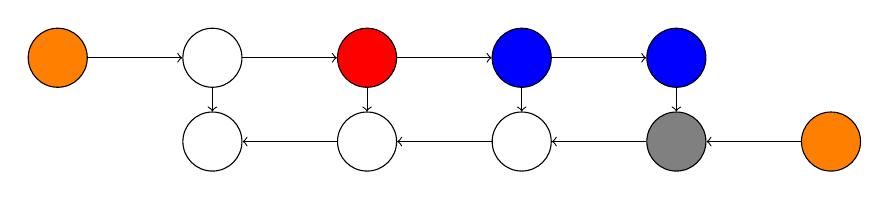
\begin{tikzpicture}[
    node distance=0.3cm and 1.2cm,
    every node/.style={circle, draw, minimum size=0.75cm},
    orange/.style={fill=orange},
    red/.style={fill=red},
    blue/.style={fill=blue},
    gray/.style={fill=gray},
    font=\small
]

\node[orange] (n1) {};
\node[right=of n1] (n2) {};
\node[red, right=of n2] (n3) {};
\node[blue, right=of n3] (n4) {};
\node[blue, right=of n4] (n5) {};

\draw[->] (n1) -- (n2);
\draw[->] (n2) -- (n3);
\draw[->] (n3) -- (n4);
\draw[->] (n4) -- (n5);

\node[below=\ysep of n2] (n6) {};
\node[below=\ysep of n3] (n7) {};
\node[below=\ysep of n4] (n8) {};
\node[gray, below=\ysep of n5] (n9) {};
\node[orange, right=1.2cm of n9] (n10) {};

\draw[->] (n7) -- (n6);
\draw[->] (n8) -- (n7);
\draw[->] (n9) -- (n8);
\draw[->] (n10) -- (n9);

\draw[->] (n2) -- (n6);
\draw[->] (n3) -- (n7);
\draw[->] (n4) -- (n8);
\draw[->] (n5) -- (n9);

\end{tikzpicture}
};
\node[above left=0.5cm and -2.5cm of seqckpt, draw=none, ] (t2) {Sequential Checkpointing};

\def\legendS{0.2cm}
\def\legendSep{-0.5}
\node[above right=-3.0cm and 1cm of plain, draw] (legend) {
  \begin{tikzpicture}
\normalsize
\fill[orange] (0,0) circle (\legendS);
\node[right] at (0.6,0) {Stored in-memory};

\fill[gray] (0,\legendSep) circle (\legendS);
\node[right] at (0.6,\legendSep) {To be computed};

\draw[thick] (0,2*\legendSep) circle (\legendS);
\fill[white] (0,2*\legendSep) circle (\legendS);
\node[right] at (0.6,2*\legendSep) {Activation};

\draw[thick] (0,3*\legendSep) circle (\legendS);
\fill[red] (0,3*\legendSep) circle (\legendS);
\node[right] at (0.6,3*\legendSep) {Checkpoint};

\draw[thick] (0,4*\legendSep) circle (\legendS);
\fill[blue] (0,4*\legendSep) circle (\legendS);
\node[right] at (0.6,4*\legendSep) {Re-computed};
\end{tikzpicture}
};


\end{tikzpicture}
\end{document}

